\begin{frame}{Μετά το \texttt{sm2} τι;}


  \definecolor{g}{RGB}{0 150 0}
  \definecolor{r}{RGB}{180 0 0}
  \definecolor{gr}{RGB}{127 127 127}


  \noindent\makebox[\linewidth][c]{%
  \begin{minipage}{\linewidth}
    \begin{figure}\centering
      \resizebox{8cm}{!}{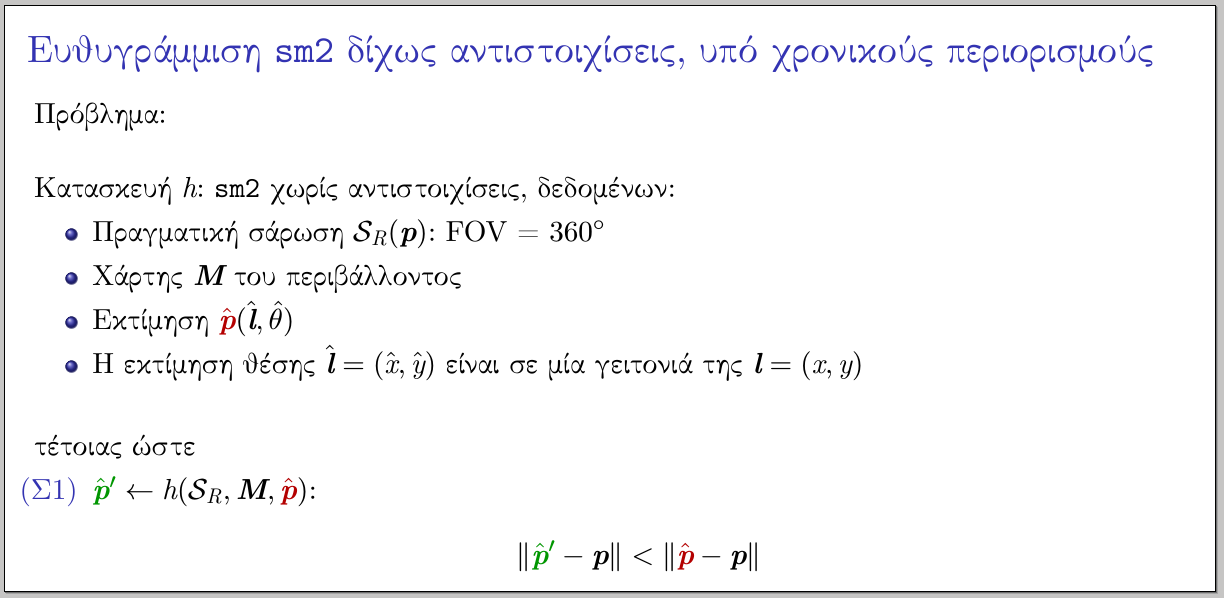
\includegraphics{./figures/slides/ch7/sm2_prob.png}}
      \begin{textblock}{14}(3.35,5.14)
        $\rightarrow \mathcal{S}_R(\bm{p})$
      \end{textblock}
      \begin{textblock}{14}(3.4,5.8)
        $\bigl\} \mathcal{S}_V(\hat{\bm{p}}_0)$
      \end{textblock}
      \begin{textblock}{14}(3.7,6.6)
        $\|\bm{\hat{\bm{l}}}_0-\bm{l}\| < \delta$
      \end{textblock}
    \end{figure}
  \end{minipage}
  }

  \noindent\makebox[\linewidth][c]{%
  \begin{minipage}{\linewidth}
    Εάν $\|\bm{\hat{\bm{l}}}_N-\bm{l}\| \ll \delta$ τότε
    \begin{itemize}
      \item $\|\bm{\hat{\bm{l}}}_{0:N}-\bm{l}\| < \delta$
      \item $\mathcal{S}_V(\hat{\bm{p}}_0) \text{ τοπική προσέγγιση } \bm{M}$ (άρα $\bm{W}$) \vspace{-0.1cm}
      \item[] στη γειτονιά της $\bm{p}, \ \forall \hat{\bm{p}}_i, i = 0,1,\dots,N$
            \makebox(0,0){\put(0,4.7\normalbaselineskip){$\left.\rule{0pt}{2.0\normalbaselineskip}\right\}$
            $\bm{M} \leftarrow \mathcal{S}_V(\hat{\bm{p}}_0) \hspace{0.25cm} \Rightarrow h$ λύνει \texttt{sm};
            }}
    \end{itemize}
  \end{minipage}
  }




\end{frame}
